\documentclass[11pt]{article}
\usepackage[margin=1in]{geometry}
\usepackage{amsmath,amssymb}
\usepackage{booktabs}
\usepackage{array}
\usepackage{graphicx}
\usepackage[colorlinks=true,linkcolor=blue,citecolor=blue,urlcolor=blue]{hyperref}

%================================================================
%  A ladder of models for inverse bremsstrahlung absorption (version 3).
%  C. K. Watson, 12 October 2026.  Build: latexmk -pdf ib_ladder_v3.tex
%  The figures (v2_fig.pdf, v3_fig.pdf) were generated by the scripts that
%  computed the numbers; every number in the text was checked by script to
%  its last printed digit.
%================================================================

\numberwithin{equation}{section}
\setlength{\emergencystretch}{3em}
\newcolumntype{L}[1]{>{\raggedright\arraybackslash}p{#1}}
\newcommand{\dd}{\mathrm d}
\newcommand{\kB}{k_B}
\newcommand{\nueff}{\nu_{\rm eff}}
\newcommand{\vos}{v_{\rm os}}

\title{A ladder of models for inverse bremsstrahlung absorption}
\author{Cooper K.\ Watson}
\date{October 12, 2026 (version 3)}

\begin{document}
\maketitle

\begin{abstract}
\noindent
The interatomic potential was built as a ladder: Coulomb, then Yukawa, which screens
it, then Lennard-Jones, which adds a repulsive core, each rung keeping the one below
as a limit and adding one physical length. Inverse bremsstrahlung (IB) absorption is
organized the same way here, from the Drude model with the Spitzer logarithm through the
quantum logarithm, screening by the electrons, the correlations of the ions, strong
collisions and their cross term with the medium, the non-Maxwellian distribution, speckles,
strong fields and the anisotropy; for neutral atoms through exact phase shifts,
polarization bremsstrahlung and multiple collisions. The correlations of the ions are computed in the hypernetted-chain
approximation for the ion mixture; for hydrogen they equal Debye--H\"uckel to
$2\times10^{-4}$, and with them the medium lowers the absorption of the nitrogen--hydrogen
mixtures by 2 to 7\,\%. The anisotropy of the heated distribution is computed with two logarithms and
electron--electron collisions and lowers the absorption by 0.8 to 1.3\,\% for hydrogen. The
heaters' own strong-field factor and the exact factor at $\vos\ge v_t$ are computed. In argon
the single-collision photon exchange beyond the formula of Kroll and Watson is computed
exactly and equals double scattering in the target at $2$ to $7\times10^{13}$~cm$^{-3}$. Applied
to the fourteen shots of Turnbull et al., the ladder, with no fitted parameter, gives
$0.96\pm0.04$ of the measured absorption for the ten nitrogen--hydrogen shots and
$1.19\pm0.06$ for the four hydrogen shots. The residual is confined to hydrogen, where every
rung of the theory is small.
\end{abstract}

\section{The idea}
\label{sec:idea}

{\noindent}(1) Every IB model in use is the Drude absorption coefficient with a
collision frequency \cite{Atzeni2004},
\begin{equation}
K=\frac{\nueff}{c}\,\frac{\omega_p^2}{\omega^2}\,\Big(1-\frac{\omega_p^2}{\omega^2}\Big)^{-1/2},
\label{eq:K}
\end{equation}
and the models differ only in $\nueff$. For electrons on ions of charge $Ze$,
\begin{equation}
\nueff=\nu_T\,\Lambda,\qquad
\nu_T=\frac{4\sqrt{2\pi}}{3}\,\frac{n_iZ^2e^4}{m^{1/2}(\kB T_e)^{3/2}},
\label{eq:nuT}
\end{equation}
and everything sits in the dimensionless ``logarithm'' $\Lambda$ and in factors
multiplying it. For electrons on neutral atoms $\nueff$ is built from the
cross sections of the atom.

{\noindent}(2) Each rung below has four parts: the formula, the effect it adds,
the dimensionless parameter that says when the effect matters, and its size at the
reference conditions. Each rung reduces to the rung below when its parameter goes
to zero. Gaussian units are used.

{\noindent}(3) \emph{The plasma reference.} Turnbull et al.\ measured the absorption
of a 527-nm probe beam in gas-jet plasmas heated by thirteen 351-nm beams, with the plasma
conditions from Thomson scattering \cite{Turnbull2023,Turnbull2024}. Of their fifteen analysed
shots, fourteen have published profiles: four in hydrogen and ten in a mixture of 43\,\% nitrogen
and 57\,\% hydrogen nuclei. All are read at the density peak of their profiles
(Tables~\ref{tab:shots} and \ref{tab:mixshots}). The probe carried 1 to 4~J in 100~ps over a
165-$\mu$m spot, about $10^{14}$~W\,cm$^{-2}$, so that at the late shots the Langdon parameter is
the probe's own; at the co-timed shots the probe carries the share $w_p$ of the overlapped
intensity. The Langdon parameter $\alpha$ is computed from the 351-nm-equivalent intensity
plotted by Turnbull et al.; it agrees with the one that Matte's formula gives from their plotted
exponent $m$ to 5.2\,\% at every shot. Their composite, the exact (Sommerfeld) logarithm and
the Langdon factor with the velocity-dependent Gaunt factor, without their screening factor,
exceeds the measured absorption by a factor $1.29\pm0.06$ for the hydrogen shots and
$1.07\pm0.04$ for the mixture shots, the averages and spreads they quote \cite{Turnbull2024}. The
\emph{hydrogen point}, $n_e/n_c=0.020$, $T_e=0.36$~keV, $T_i=0.05$~keV, serves for the rungs that
do not depend on the field. \emph{The gas reference} is argon, the main constituent of one fill
of an electron-beam-pumped KrF laser, at electron temperatures of 300~K and 1.08~eV and at 1, 4
and 28.3~THz.

\begin{table}[ht]
\caption{The four hydrogen shots of Turnbull et al.\ \cite{Turnbull2024} at the density
peak: probe time, $n_e/n_c$ at 527~nm, $T_e$, the Langdon parameter $\alpha$, the probe's share
$w_p$ of the intensity, and $u=\hbar\omega/\kB T_e$. The ion temperature is 0.05~keV.}
\label{tab:shots}
\begin{center}
\begin{tabular}{ccccccc}
\toprule
shot & $t_{\rm probe}$ (ns) & $n_e/n_c$ & $T_e$ (keV) & $\alpha$ & $w_p$ & $u$\\
\midrule
102727 & 0.6 & 0.0177 & 0.37 & 0.044 & 1 & 0.00636\\
104031 & 0.3 & 0.0229 & 0.34 & 0.119 & 0.27 & 0.00692\\
106310 & 0.3 & 0.0100 & 0.26 & 0.180 & 0.29 & 0.00905\\
106311 & 0.3 & 0.0047 & 0.20 & 0.232 & 0.29 & 0.01177\\
\bottomrule
\end{tabular}
\end{center}
\end{table}

\begin{table}[ht]
\caption{The ten nitrogen--hydrogen shots of Turnbull et al.\ \cite{Turnbull2024} at the density
peak: probe time, $n_e/n_c$, $T_e$, $T_i$, the nitrogen charge $Z_N$ used in their calculations,
$Z_{\rm eff}=\langle Z^2\rangle/\langle Z\rangle$, the coupling $\Gamma_{NN}$ of the nitrogen ions,
$\alpha$ and $w_p$.}
\label{tab:mixshots}
\begin{center}
\begin{tabular}{ccccccccc}
\toprule
shot & $t_{\rm probe}$ (ns) & $n_e/n_c$ & $T_e$ (keV) & $T_i$ (keV) & $Z_N$ & $Z_{\rm eff}$ & $\Gamma_{NN}$ & $\alpha$ ($w_p$)\\
\midrule
102729 & 0.6 & 0.0149 & 0.65 & 0.070 & 6.5 & 5.57 & 0.276 & 0.086 (1.00)\\
102737 & 0.3 & 0.0179 & 0.42 & 0.050 & 5 & 4.16 & 0.261 & 0.189 (0.40)\\
102738 & 0.3 & 0.0189 & 0.70 & 0.070 & 6 & 5.10 & 0.260 & 0.547 (0.15)\\
104035 & 0.3 & 0.0179 & 0.62 & 0.070 & 5 & 4.16 & 0.186 & 0.299 (0.23)\\
104037 & 0.6 & 0.0179 & 0.62 & 0.100 & 6 & 5.10 & 0.179 & 0.067 (1.00)\\
104041 & 0.6 & 0.0194 & 0.43 & 0.090 & 6 & 5.10 & 0.204 & 0.108 (1.00)\\
106315 & 0.6 & 0.0184 & 0.63 & 0.090 & 6 & 5.10 & 0.201 & 0.147 (1.00)\\
106316 & 0.6 & 0.0080 & 0.45 & 0.045 & 5.5 & 4.63 & 0.261 & 0.150 (1.00)\\
106317 & 0.6 & 0.0039 & 0.30 & 0.030 & 5 & 4.16 & 0.261 & 0.196 (1.00)\\
106319 & 0.6 & 0.0279 & 0.80 & 0.120 & 7 & 6.04 & 0.225 & 0.086 (1.00)\\
\bottomrule
\end{tabular}
\end{center}
\end{table}

\section{The electron--ion ladder}
\label{sec:plasma}

\subsection{Drude--Spitzer}
\label{sec:drude}
The classical logarithm $\Lambda=\ln(b_{\max}/b_{\min})$ with the Debye length
$b_{\max}=\lambda_{De}=v_t/\omega_p$ and $b_{\min}$ the larger of the
$90^\circ$ impact parameter $Ze^2/3\kB T_e$ and the de Broglie length $\hbar/2mv$,
both at $mv^2=3\kB T_e$ \cite{Atzeni2004}; $v_t=(\kB T_e/m)^{1/2}$. This is the
``Coulomb potential'' of the ladder: right in form, with cutoffs put in by hand.
At the hydrogen point $\lambda_{De}=15.73$~nm, the de Broglie length
$0.2887\,\hbar/mv_t=4.20\times10^{-3}$~nm exceeds $Ze^2/3\kB T_e=1.33\times10^{-3}$~nm,
and $\Lambda_0=8.23$.

\subsection{The quantum logarithm}
\label{sec:quantum}
Second order in the ion potential, with Volkov (field-dressed) electron states and a
Maxwell distribution, gives the collision frequency of Eq.~\eqref{eq:nuT} with
\begin{equation}
\Lambda_1(u)=\frac{1-e^{-u}}{u}\,e^{u/2}K_0\Big(\frac u2\Big),\qquad u=\frac{\hbar\omega}{\kB T_e},
\label{eq:Lam1}
\end{equation}
absorption net of stimulated emission, and no cutoff. This is Kramers' result with the
Born Gaunt factor, $\Lambda_1=(\pi/\sqrt3)\langle g_B\rangle(1-e^{-u})/u$ with
$\langle g_B\rangle=(\sqrt3/\pi)e^{u/2}K_0(u/2)$ \cite{Kramers1923,KarzasLatter1961}.
For $u\ll1$, $K_0(x)=-\ln(x/2)-\gamma+O(x^2\ln x)$ gives
\begin{equation}
\Lambda_1\simeq\ln\frac{4\kB T_e}{e^\gamma\hbar\omega}=\ln\frac{b_{\max}}{b_{\min}},\qquad
b_{\max}=\frac{v_t}{\omega},\qquad b_{\min}=\frac{e^\gamma}{4}\,\frac{\hbar}{mv_t}=0.445\,\frac{\hbar}{mv_t},
\label{eq:cutoffs}
\end{equation}
with $\gamma$ Euler's constant. The theory fixes both cutoffs. The upper one is the
distance an electron travels in a radian of the laser period, the dynamic cutoff of
Dawson and Oberman \cite{DawsonOberman1962}, not the Debye length. This is the
``Yukawa'' step: the long range is cut by a physical length. Parameter: $\omega/\omega_p$
for the upper cutoff, $u$ for the photon energy. At the hydrogen point
$b_{\max}=2.225$~nm and $\Lambda_1=5.84$. The logarithm $\Lambda_0$ of Sec.~\ref{sec:drude} exceeds it by $\ln(\omega/\omega_p)+\ln(0.445/0.2887)=1.96+0.43$,
or 40.9\,\%, in line with the finding of Turnbull et al.\ that transport logarithms with a
Debye length miss their data by more than 50\,\% \cite{Turnbull2023}.

\subsection{Dynamic screening by the electrons}
\label{sec:escreen}
With the electrons' own response, second order in the ion potential gives the
high-frequency collision frequency of Dawson and Oberman \cite{DawsonOberman1962},
\begin{equation}
\nueff=-\frac{2Ze^2}{3\pi m\omega}\int_0^\infty k^2S(k)\,{\rm Im}\,\frac{1}{\varepsilon(k,\omega)}\,\dd k,
\label{eq:DO}
\end{equation}
with $\varepsilon$ the longitudinal dielectric function of the electrons and $S$ the
static structure factor of the ions. For bare ions ($S=1$) and the quantum (Lindhard)
dielectric function of Maxwell electrons, with $x=kv_t/\omega$ and $r=\omega_p/\omega$,
\begin{equation}
\Lambda_2=-\frac{1}{r^2}\Big(\frac2\pi\Big)^{1/2}\int_0^\infty x^2\,{\rm Im}\,\frac{1}{\varepsilon(x)}\,\dd x,\qquad
\varepsilon(x)=1-\frac{r^2}{\sqrt2\,ux^3}\big[Z(\zeta_+)-Z(\zeta_-)\big],\quad
\zeta_\pm=\frac{1}{\sqrt2}\Big(\frac1x\pm\frac{ux}{2}\Big),
\label{eq:Lam2}
\end{equation}
where $Z$ is the plasma dispersion function. Replacing ${\rm Im}\,\varepsilon^{-1}$ by
$-{\rm Im}\,\varepsilon$ gives back Eq.~\eqref{eq:Lam1}. Parameter: $r=\omega_p/\omega$.
At the hydrogen point the electrons lower the logarithm by 0.0076, or 0.13\,\%.

\subsection{Correlations of the ions}
\label{sec:ions}
The ions enter Eq.~\eqref{eq:DO} only through $S(k)$. Their mean spacing does not appear
by itself; uncorrelated ions add whatever their spacing. In a weakly coupled plasma
$S$ has the Debye--H\"uckel form
\begin{equation}
S(k)=\frac{k^2+k_{De}^2}{k^2+k_{De}^2+k_{Di}^2},\qquad k_{Di}^2=a\,k_{De}^2,\qquad a=\frac{ZT_e}{T_i}.
\label{eq:Sdh}
\end{equation}
With static (Debye) electrons and soft photons the ion term has a closed form. The
one-speed logarithm changes by $\int_{\omega/v}^\infty[S(q)-1]\,\dd q/q
=-(k_{Di}^2/2k_t^2)\ln(1+k_t^2v^2/\omega^2)$, $k_t^2=k_{De}^2+k_{Di}^2$, and the
Maxwell average, with $\int_0^\infty e^{-s}\ln(1+\kappa s)\,\dd s=e^{1/\kappa}E_1(1/\kappa)$, gives
\begin{equation}
\Delta\Lambda_3\simeq\bar I=-\frac{a}{2(1+a)}\,e^{1/\kappa}E_1(1/\kappa),\qquad
\kappa=2(1+a)\,\frac{n_e}{n_c}.
\label{eq:Ibar}
\end{equation}
Parameters: $k_{Di}/k_{De}=a^{1/2}$ for the size, and the ion coupling
$\Gamma_{ii}=Z^2e^2/a_i\kB T_i$ for the validity of Eq.~\eqref{eq:Sdh}, with
$a_i=(3/4\pi n_i)^{1/3}$. At the hydrogen point $a=7.2$, $\kappa=0.328$ and
$\Gamma_{ii}=0.020$. Equation~\eqref{eq:DO} with Eq.~\eqref{eq:Sdh} and the Lindhard
$\varepsilon$ lowers the logarithm by a further 0.114, or 1.96\,\%; Eq.~\eqref{eq:Ibar}
gives $-0.1136$, within 0.44\,\% of it. With the electron screening of Sec.~\ref{sec:escreen}, the medium lowers $\Lambda_1$ by
2.08\,\%. At the four shots the medium factor $\Lambda_{2,3}/\Lambda_1$ is 0.981, 0.978,
0.991 and 0.996 (Table~\ref{tab:budget}); it would be 0.968 at the first shot with
$T_i=0.025$~keV and 0.989 with 0.1~keV.

{\noindent}\emph{Against the fitted factor.} Turnbull et al.\ multiply the absorption by
$f_{sc}=\{\ln[(2\kB T_e/\hbar\omega)\,y/(1+y^2)^{1/2}]-1/[2(1+y^2)]\}/\ln(2\kB T_e/\hbar\omega)$,
$y=l_{sc}\omega/v_t$, the Born logarithm of a Yukawa ion of screening length $l_{sc}$
\cite{Turnbull2023}. With $l_{sc}=\lambda_{D,ei}=5.49$~nm, the Debye length of electrons
and ions, it lowers the absorption by 2.56\,\%, close to the medium of Secs.~\ref{sec:escreen} and \ref{sec:ions}. With the interionic
distance $l_{sc}=a_i=1.437$~nm, chosen to match their data, it lowers it by 16.8\,\%,
about eight times what the medium gives.

{\noindent}\emph{Beyond Debye--H\"uckel.} Equation~\eqref{eq:Sdh} is the weak-coupling limit. The
structure factor of an ion mixture follows at any coupling from the Ornstein--Zernike relation
with the hypernetted-chain closure \cite{Morita1958}. With ions $i$ of charge $Z_ie$ and density
$n_i$ at the temperature $T_i$, interacting through the electron-screened potential
$\phi_{ij}=Z_iZ_je^2e^{-k_{De}r}/r$,
\begin{equation}
h_{ij}(r)=\exp\Big[-\frac{\phi_{ij}(r)}{\kB T_i}+h_{ij}(r)-c_{ij}(r)\Big]-1,\qquad
\tilde h_{ij}(k)=\tilde c_{ij}(k)+\sum_l\tilde c_{il}(k)\,n_l\,\tilde h_{lj}(k),
\label{eq:hnc}
\end{equation}
and the absorption takes the charge structure factor
\begin{equation}
S_{ZZ}(k)=\frac{\sum_in_iZ_i^2+\sum_{ij}n_in_jZ_iZ_j\tilde h_{ij}(k)}{\sum_in_iZ_i^2}
\label{eq:SZZ}
\end{equation}
in place of $S$ in Eq.~\eqref{eq:DO}. The equations are solved by iteration on a radial grid, with the
long-range parts of $c_{ij}$ and $h_{ij}-c_{ij}$ subtracted and transformed analytically, so that
the Debye--H\"uckel solution is the exact starting point. For the one-component plasma the
excess energy is $-0.5704$ at $\Gamma=1$, against $-0.5726$ from the Monte Carlo fit of Slattery,
Doolen and DeWitt \cite{Slattery1982}, and $-0.02569$ at $\Gamma=0.1$, against $-0.02590$ from Abe's
expansion \cite{Abe1959} and $-0.02739$ from Debye--H\"uckel. At the hydrogen point the
hypernetted-chain $S$ differs from Eq.~\eqref{eq:Sdh} by at most $6.2\times10^{-4}$, and at the four
hydrogen shots the medium factor changes by at most $1.9\times10^{-4}$: for hydrogen the correlations
beyond Debye--H\"uckel are nil. The mixtures are another matter. There
$k_{Di}^2/k_{De}^2=Z_{\rm eff}T_e/T_i$ is 24 to 52 and $\Gamma_{NN}=0.18$ to 0.28, the medium factor is 0.930 to 0.982, and the
hypernetted chain raises it by 0.0037 to 0.0064 against Debye--H\"uckel. The medium lowers the
absorption by 2 to 7\,\% in the mixtures and by 0.4 to 2.2\,\% in hydrogen. Halving or
doubling $T_i$, the least certain reading, moves the mixture medium factor between 0.904 and 0.989.
The fitted factor of Turnbull et al., with the interionic distance of the nitrogen ions for the
mixtures as they use it and of the protons for hydrogen, is 0.879 to 0.969 for the mixtures and
0.827 to 0.927 for hydrogen; at the density peaks it reproduces their reported changes
$1.29\to1.13$ and $1.07\to1.00$ to 0.8 and 2.3\,\%.

\subsection{Strong collisions}
\label{sec:strong}
The Born approximation needs $\eta=Ze^2/\hbar v\ll1$. The exact Coulomb (Sommerfeld)
free--free Gaunt factor removes that condition \cite{Sommerfeld1931,KarzasLatter1961}:
\begin{equation}
\Lambda_4=\frac{\pi}{\sqrt3}\,\langle g\rangle(\gamma^2,u)\,\frac{1-e^{-u}}{u},\qquad
\gamma^2=\frac{Z^2\,{\rm Ry}}{\kB T_e}=\frac{\eta_t^2}{2},\quad \eta_t=\frac{Ze^2}{\hbar v_t},
\label{eq:Lam4}
\end{equation}
with the thermally averaged exact Gaunt factor $\langle g\rangle$ tabulated by van Hoof et
al.\ \cite{vanHoof2014}. As $\gamma^2\to0$ it tends to $\langle g_B\rangle$ and $\Lambda_4$ to
$\Lambda_1$. In the soft-photon limit the exact logarithm of one electron is the Born one
plus Bloch's constant $\Delta(\eta)=-\gamma-{\rm Re}\,\psi(1+i\eta)$ \cite{Bloch1933}, which is
$-\zeta(3)\eta^2$ for $\eta\ll1$ and $-\gamma-\ln\eta$ for $\eta\gg1$, where it turns the
quantum lower cutoff into the classical one. Parameter: $\eta_t$. At the hydrogen point
$\eta_t=0.275$ and $\langle g\rangle/\langle g_B\rangle=0.99315$, a correction of
$-0.685$\,\%; at the four shots it is $-0.67$ to $-0.88$\,\%. For fully stripped nitrogen
($Z=7$) at the same $T_e$ and $u$, $\eta_t=1.92$ and the correction is $-15.4$\,\%.

{\noindent}\emph{The cross term with the medium.} The exact correction is added to the
logarithm of Sec.~\ref{sec:ions}, $\Lambda_{2,3}+(\Lambda_4-\Lambda_1)$. Whether the medium changes the
strong-collision correction itself is decided by the partial waves of an ion screened to
$V=-(Ze^2/r)e^{-r/\lambda}$. In the soft-photon limit the logarithm of one electron is the
transport sum $S=\sum_l(l+1)\sin^2(\delta_{l+1}-\delta_l)$ of its phase shifts, cut at the
partial wave $J=kb_{\max}=k^2/\omega$ of the dynamic cutoff, in units of $\eta^2$; with
the first Born phases, $S^B=\sum_l(l+1)(\delta^B_{l+1}-\delta^B_l)^2$. For the bare Coulomb
field $\delta_l={\rm ph}\,\Gamma(l+1-i\eta)$, $\delta^B_l=-\eta\psi(l+1)$, and
$(S-S^B)/\eta^2=\Delta(\eta)+O(\eta^2/J^2)$ exactly. For the screened field the exact
phases come from the radial equation, integrated numerically, and the Born phases are
$\delta^B_l=\eta\,Q_l(1+1/2k^2\lambda^2)$ with the Legendre function of the second kind.
The cross term
\begin{equation}
C=\frac{S^Y-S^{Y,B}}{\eta^2}-\frac{S^C-S^{C,B}}{\eta^2}
\label{eq:cross}
\end{equation}
is the part of the exact-minus-Born correction that the screening changes; the Born part
of the screening, $(S^{Y,B}-S^{C,B})/\eta^2$, is the second-order medium of Sec.~\ref{sec:ions} and is not
in $C$. For the Coulomb field only odd powers of $\eta$ enter the phases, so there is no
second-Born term in their differences; for the screened field there is, and $C$ is
first order in $b_{\max}/\lambda$, not in $b_{90}/\lambda$ as the size of the strong-collision region
would suggest.
Averaged over the Maxwellian with the soft-photon weight $e^{-s}$, $s=E/\kB T_e$, at
$T_e=0.36$~keV: for hydrogen $\langle C\rangle=+0.0098$ with $\lambda=\lambda_{D,ei}=5.49$~nm
and $+0.0035$ with $\lambda=\lambda_{De}=15.73$~nm, against $\langle\Delta\rangle=-0.134$ for the
bare ion, that is 7.4\,\% and 2.6\,\% of the strong-collision correction and
$1.7\times10^{-3}$ and $6.0\times10^{-4}$ of $\Lambda_1$. For $Z=7$,
$\langle C\rangle=+0.0359$ and $+0.0128$ against $\langle\Delta\rangle=-1.235$, that is 2.9\,\%
and 1.0\,\% of the correction and $6.1\times10^{-3}$ and $2.2\times10^{-3}$ of $\Lambda_1$.
The sign is positive: the medium weakens the strong-collision correction. Doubling the
cutoff $J$ changes $C$ by 9\,\% at $s=0.25$ and by 2 to 3\,\% at $s\ge1.2$. The soft-photon
average $\langle\Delta\rangle$ overstates the exact thermal correction of Eq.~\eqref{eq:Lam4} by a factor
3.3 for hydrogen, since the slow electrons, for which the photon is not soft, are
focused by the ion; $C$ shares that weighting, so these are upper values. In the
absorption the cross term is below 0.2\,\% for hydrogen and about 0.6\,\% for the
nitrogen ions of the mixed shots. At the conditions of the mixture shots, $Z=6$, $T_e=0.62$~keV and the total screening length
$\lambda_t=3.58$~nm of shot 106315, $\langle C\rangle=+0.0383$ against $\langle\Delta\rangle=-0.870$,
$6.0\times10^{-3}$ of $\Lambda_1$. This closes the item.

\subsection{The non-Maxwellian distribution (Langdon)}
\label{sec:langdon}
IB heats slow electrons fastest. When it outpaces the electron--electron collisions the
distribution flattens toward $F\propto\exp[-(v/v_m)^M]$ with $M>2$ \cite{Langdon1980}.
The parameter is $\alpha=Z\vos^2/v_t^2$, with $\vos$ the peak quiver velocity, and Matte et
al.\ fit the exponent as $m(\alpha)=2+3/(1+1.66/\alpha^{0.724})$ \cite{Matte1988}. For an
isotropic distribution the heating rate is $P\propto-\int_0^\infty L(v)\,\partial_vF\,\dd v$,
with the one-speed Born logarithm $L(v)=\ln(2mv^2/\hbar\omega)$. At fixed $L$ this is
$LF(0)$, and the factor is $F_M(0)/F_2(0)$ at fixed density and energy; Langdon's fit
$f_L=1-0.553/[1+(0.27/\alpha)^{0.75}]$ \cite{Langdon1980} equals it at $M=m(\alpha)$ to
within 0.27\,\% for $\alpha=10^{-3}$ to $10^3$. With the velocity-dependent $L$, the
substitution $s=(v/v_m)^M$ and $\int_0^\infty e^{-s}\ln s\,\dd s=-\gamma$ give
\begin{equation}
\frac{P_M}{P_2}=\frac{F_M(0)}{F_2(0)}\;
\frac{\ln\big(2v_m^2/uv_t^2\big)-2\gamma/M}{\ln(4/u)-\gamma},\qquad
\frac{v_m^2}{v_t^2}=\frac{3\Gamma(3/M)}{\Gamma(5/M)} .
\label{eq:langdon}
\end{equation}
The second factor, one at $M=2$, raises the absorption: a flattened distribution moves
electrons to speeds where the logarithm is larger. At the four shots $m=2.18$, 2.34, 2.45
and 2.52, $f_L=0.887$, 0.806, 0.765 and 0.739, the logarithm factor $C_L$ is 1.031, 1.056,
1.072 and 1.085, and the product $f_LC_L$ is 0.914, 0.851, 0.820 and 0.802. At the mixture shots $\alpha=0.067$ to 0.547.

\subsection{Speckles}
\label{sec:speckles}
A real beam has an intensity pattern. If the distribution adjusts locally and $T_e$ is
uniform, the absorbed power is that of the mean intensity times an average of $f_L$ over
the pattern. The probe's own pattern has the exponential distribution of a fully developed
speckle field, $x=I/\langle I\rangle\sim e^{-x}$, and the probe is absorbed where its own
intensity is, with the weight $x$; the thirteen heater beams carry independent patterns,
whose sum $y$ has the gamma distribution of shape 13 and mean one. With $\alpha_p=w_p\alpha$
and $\alpha_h=(1-w_p)\alpha$,
\begin{equation}
f_{sp}=\int_0^\infty\!\dd x\,x\,e^{-x}\int_0^\infty\!\dd y\,\frac{13^{13}y^{12}e^{-13y}}{12!}\,
f_L(\alpha_hy+\alpha_px).
\label{eq:fsp}
\end{equation}
Since $f_L$ falls with $\alpha$, the bright speckles absorb less per unit intensity.
Parameter: $\alpha$, and the ratio of the speckle size to the electron relaxation length
(Eq.~\eqref{eq:fsp} is the local limit; in the opposite limit $f_{sp}=f_L$). At the four
shots $f_{sp}/f_L=0.955$, 0.977, 0.973 and 0.972: the late shot, where the probe is the
only beam, is the most affected.

\subsection{Strong fields: the probe's own field and the heaters' quiver}
\label{sec:fields}
When the quiver velocity is not small against the thermal velocity the field cannot be
treated to lowest order. Second order in the ion potential but exact in the field gives the
heating rate as a sum over photon numbers $\ell$, each weighted by $J_\ell^2(\mathbf k\cdot\mathbf a_0)$
with $\mathbf a_0$ the quiver amplitude, inside the dielectric form of Secs.~\ref{sec:escreen} and \ref{sec:ions}
\cite{KullPlagne2001,Bornath2001,Decker1994}. Parameter: $\beta=\vos/v_t=(\alpha/Z)^{1/2}$.
At the four shots the probe has $\beta_p=0.21$, 0.18, 0.23 and 0.26, and the heaters
$\beta_h=0$, 0.29, 0.36 and 0.40. Two effects follow, computed here with the free-electron
response $\chi_0$ of Maxwell electrons and bare ions, in the variables $x=kv_t/\omega_p$,
$u=\hbar\omega_p/\kB T_e$ and
\begin{equation}
D(x;\nu)=e^{-\frac12(\nu/x-ux/2)^2}-e^{-\frac12(\nu/x+ux/2)^2},\qquad
\int_0^\infty D(x;1)\,\frac{\dd x}{x}=u\Lambda_1(u),
\label{eq:D}
\end{equation}
$D$ being proportional to $x\,{\rm Im}\,\chi_0(k,\nu\omega_p)$, absorption net of emission.

{\noindent}\emph{The probe alone.} With $B_\ell(z)=\int_{-1}^1J_\ell^2(z\mu)\,\dd\mu$ the exact
ratio of the probe's collision frequency to its weak-field value is
\begin{equation}
R_{\rm self}(\beta_p,u)=\frac{3}{u\beta_p^2\Lambda_1}\sum_{\ell=-\infty}^\infty\ell
\int_0^\infty\frac{\dd x}{x^3}\,D(x;\ell)\,B_\ell(x\beta_p),
\label{eq:Rself}
\end{equation}
which tends to one as $\beta_p\to0$. Its quasi-static limit at a fixed logarithm is Silin's
$1-\tfrac{9}{40}\beta_p^2+O(\beta_p^4)$; the exact coefficient at $u=0.0064$ is 0.195, smaller
because the largest momentum transfer grows with the field. At the four shots
$R_{\rm self}=0.991$, 0.994, 0.990 and 0.987.

{\noindent}\emph{The probe inside the heaters' quiver.} With two fields the quiver is
$\mathbf a(t)=\mathbf a_h\sin\omega_ht+\mathbf a_p\sin\omega_pt$, and the Volkov phase
$e^{i\mathbf k\cdot\mathbf a(t)}$ has sidebands at $\ell\omega_h+m\omega_p$ with the weights
$J_\ell^2(\mathbf k\cdot\mathbf a_h)J_m^2(\mathbf k\cdot\mathbf a_p)$; for $\omega_h/\omega_p=3/2$
no two sidebands with $|m|\le1$ coincide. The probe's photons are counted by $m$, and to
second order in the probe field only $m=\pm1$ enter, so that
\begin{equation}
R_{pp}(\psi)=\frac{\displaystyle\sum_{\ell=-\infty}^\infty\int_0^\infty\frac{\dd x}{x}\,
D\Big(x;1+\ell\frac{\omega_h}{\omega_p}\Big)\,W_\ell^\psi\Big(\frac{x\beta_h\omega_p}{\omega_h}\Big)}
{\displaystyle\frac23\int_0^\infty\frac{\dd x}{x}\,D(x;1)},
\label{eq:Rpp}
\end{equation}
\begin{equation}
W_\ell^\psi(z)=\int_{-1}^1J_\ell^2(z\mu)\Big[\frac{\sin^2\psi}{2}(1-\mu^2)+\cos^2\psi\,\mu^2\Big]\dd\mu,
\label{eq:W}
\end{equation}
with $\psi$ the angle between the two polarizations; averaged over $\psi$,
$W_\ell=B_\ell/3$, and $W_\ell^\psi(0)=\tfrac23\delta_{\ell0}$ returns the weak field. The
terms with $\ell<0$ have $1+\ell\omega_h/\omega_p<0$ and $D<0$: an electron that absorbs a
probe photon while emitting a heater photon loses energy, so the reverse process, a heater
photon absorbed and a probe photon emitted, is favoured, and the heater feeds the probe
through the ions. At large $k$ the sidebands cancel, since $\sum_\ell J_\ell^2=1$ and
$\sum_\ell\ell J_\ell^2=0$ and $D$ is linear in $\nu$ there; the effect is a logarithmic
integral from the thermal cutoff $x\sim1$ upward, of relative size $\beta_h^2$. Two
independent checks: the small-field series of Eq.~\eqref{eq:Rpp}, from
$B_0=2-z^2/3$ and $B_{\pm1}=z^2/6$, gives $R_{pp}=1-c\beta_h^2$ with $c=0.212$ averaged
over $\psi$ at $u=0.0064$, which the full sum reproduces to $6\times10^{-5}$ at
$\beta_h=0.2$; and the classical picture of ions drifting through the electron gas with
the velocity $-(\mathbf u_h+\mathbf u_p)(t)$, a drag $-h(s)\mathbf s$ with $s=u/\sqrt2v_t$
and $h=[\sqrt\pi\,{\rm erf}(s)/s-2e^{-s^2}]/s^2$, gives for the probe's power
$\langle F\cdot u_p\rangle$ to second order
$R^{qs}_{pp}(\psi)=\tfrac34\langle h(s_h)+s_hh'(s_h)\cos^2\psi\rangle$, which at small
$\beta_h$ is $1-\tfrac{9}{20}\beta_h^2$ for parallel polarizations, $1-\tfrac{3}{20}\beta_h^2$
for perpendicular ones and $1-\tfrac14\beta_h^2$ averaged. A pump is therefore twice as
effective on a probe as a beam on itself, $\tfrac{9}{40}\to\tfrac{9}{20}$, because the two
phases are independent. At $\beta_h=0.2$ the exact $1-R_{pp}$ is 0.0151, 0.0051 and 0.0084
for the three cases against 0.0178, 0.0060 and 0.0099 quasi-static, the same ratio 0.847
in all three, as for $R_{\rm self}$ against Silin. The thirteen heaters surround the
plasma, so the average over $\psi$ is the physical case. At the co-timed shots
$R_{pp}=0.982$, 0.974 and 0.967 averaged, 0.968, 0.953 and 0.941 for parallel and 0.989,
0.984 and 0.980 for perpendicular polarizations. The product $R_{\rm self}R_{pp}$ is
0.991, 0.976, 0.964 and 0.954 at the four shots. For the heater beams themselves the
single-beam factor at their own $\beta_h=0.29$, 0.36 and 0.40 is $R_{\rm self}=0.983$, 0.976 and
0.969 at the co-timed shots: the heating rate is 2 to 3\,\% below its weak-field value. At
$\beta\ge1$ Eq.~\eqref{eq:Rself} at $u=0.0064$ gives 0.953, 0.828 and 0.507 for $\beta=0.5$, 1 and
2, against Silin's 0.946, 0.805 and 0.460: the exact rate exceeds the quasi-static one by 1, 3
and 10\,\%, because the largest momentum transfer grows with the quiver velocity. This closes the
item.

\begin{figure}[ht]
\centering
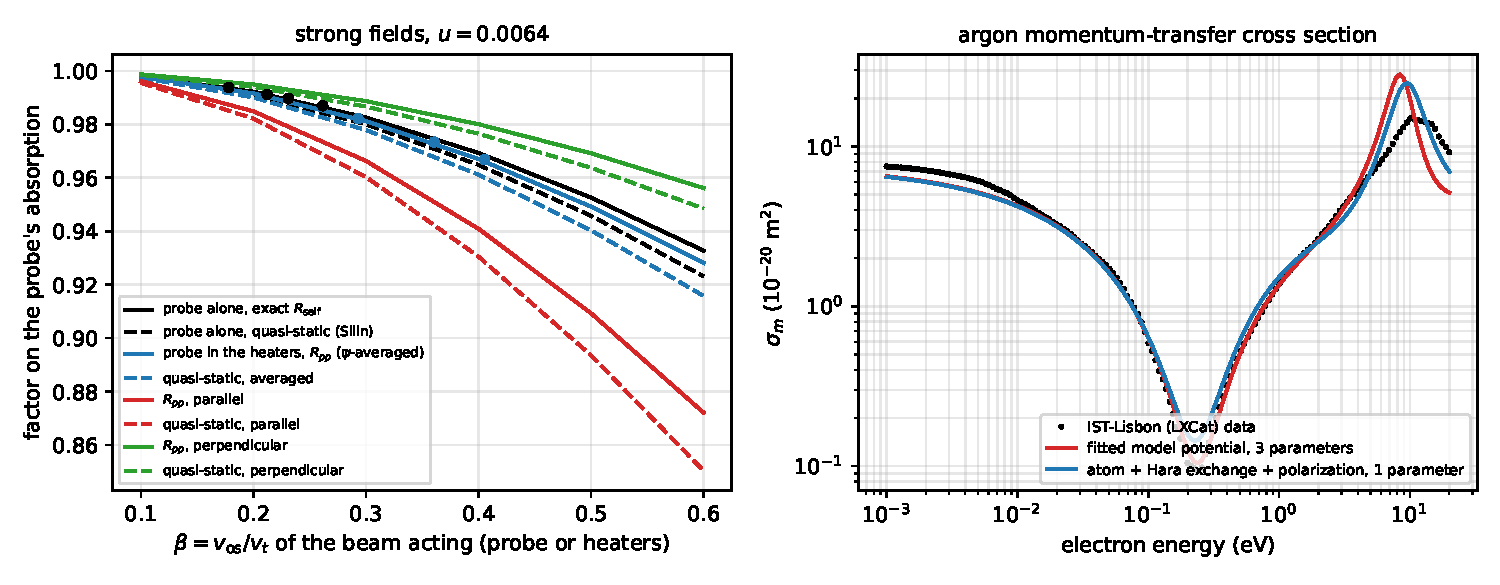
\includegraphics[width=\textwidth]{v2_fig.pdf}
\caption{Left: the strong-field factors on a probe's absorption at $u=0.0064$ against
$\beta=\vos/v_t$ of the beam that acts. Black: the probe's own field, exact
(Eq.~(\ref*{eq:Rself})) and quasi-static (Silin). Colours: the probe inside the heaters'
quiver, Eq.~(\ref*{eq:Rpp}), averaged over the polarizations (blue), parallel (red) and
perpendicular (green), exact (solid) and in the quasi-static drag picture (dashed). Dots:
the four hydrogen shots. Right: the momentum-transfer cross section of argon from the
IST-Lisbon data, from the three-parameter model potential of Eq.~(\ref*{eq:model}), and from
the Hartree--Fock atom with Hara's exchange and one fitted cutoff.}
\label{fig:v2}
\end{figure}

\subsection{The anisotropy}
\label{sec:aniso}
A linearly polarized field heats along its polarization, and the distribution acquires a
part of degree 2 in the angle, $f=f_0+f_2(v)P_2(\hat{\mathbf v}\cdot\boldsymbol\epsilon)$. Its direct
effect on the absorption of the same beam is
\begin{equation}
\frac{\delta P}{P}=-\frac25\,\frac{\vos^2}{v_t^2}\,Q,\qquad
Q=\int_0^\infty\frac{f_2(v)}{(\vos^2/3v_t^2)\,f_0(0)}\,\frac{\dd v}{v},
\label{eq:aniso}
\end{equation}
with $\vos$ the probe's own quiver velocity. In the Lorentz limit, $Z\gg1$, the field drives $f_2$
through the ion collisions and the same collisions relax it, $f_2=S_2/3\nu_{ei}$, and for the
self-similar heated distribution $Q$ is a number of order one, 1.32, 1.03, 0.93 and 0.87 at the
$\alpha$ of the four shots. Two corrections enter. The drive is inverse bremsstrahlung and carries
the logarithm $\Lambda_1$ with the dynamic cutoff, while the relaxation of the quasi-static $f_2$ is
pitch-angle scattering and carries the transport logarithm $\ln(\lambda_{De}/b_{\min})$ of Sec.~\ref{sec:drude}, 8.10 to
8.36 at the shots: $f_2$ is smaller by $\Lambda_1/\Lambda_{\rm tr}=0.63$ to 0.71. And at $Z=1$ the
electron--electron collisions relax $f_2$ as well. With the test-particle collision operator on a
Maxwellian background \cite{Rosenbluth1957}, in units of $4\pi n_ee^4\Lambda_{\rm tr}/m^2v_t^3$ and with
$w=v/v_t$, $x=w^2/2$ and $\psi(x)={\rm erf}\sqrt x-2(x/\pi)^{1/2}e^{-x}$, $f_2$ solves
\begin{equation}
3\Big(\frac{Z}{w^3}+\nu_D\Big)f_2-\frac{1}{w^2}\frac{\dd}{\dd w}\Big[w^2\frac{\psi}{w^3}\Big(\frac{\dd f_2}{\dd w}+wf_2\Big)\Big]
=\frac{3Z}{w^3}\,\frac{\Lambda_1}{\Lambda_{\rm tr}}\,S_2,\qquad
\nu_D=\frac{(1-1/2x)\psi+\psi'}{w^3},
\label{eq:f2ee}
\end{equation}
with the drive $S_2$ of the Lorentz limit. The operator keeps the Maxwellian, and for fast
electrons at $Z=1$ the deflection by electrons equals that by ions, as it must \cite{Spitzer1953}.
For a Maxwellian drive the electron--electron collisions lower $Q$ by a factor 0.77 to 0.80 at the
hydrogen shots and 0.94 to 0.96 at the mixture shots, where $Z_{\rm eff}\approx5$. Applied to the
self-similar $Q$, the direct effect is 1.30, 0.76, 1.02 and 1.15\,\% at the four hydrogen shots,
against 2.3, 1.3, 2.0 and 2.4\,\% in the Lorentz limit with one logarithm, and 0.32 to 1.07\,\% at the
mixture shots. The feedback of $f_2$ on the isotropic part and the field-particle part of the
electron--electron operator are not computed; the direct part is.

\subsection{The plasma ladder at the hydrogen point}
\label{sec:hpoint}

\begin{table}[ht]
\caption{The electron--ion ladder at the hydrogen point ($n_e/n_c=0.020$, $T_e=0.36$~keV,
$T_i=0.05$~keV, 526.7~nm). The logarithm after each rung and its change against $\Lambda_1$.}
\label{tab:plasma}
\begin{center}
\begin{tabular}{lL{4.6cm}ccc}
\toprule
Sec. & Adds & Parameter & $\Lambda$ & against $\Lambda_1$ (\%)\\
\midrule
\ref*{sec:drude} & Drude--Spitzer, cutoffs by hand & --- & 8.228 & $+40.9$\\
\ref*{sec:quantum} & quantum logarithm, dynamic cutoff & $u$, $\omega/\omega_p$ & 5.839 & 0\\
\ref*{sec:escreen} & screening by the electrons & $\omega_p/\omega$ & 5.832 & $-0.13$\\
\ref*{sec:ions} & correlations of the ions & $a^{1/2}$, $\Gamma_{ii}$ & 5.717 & $-2.08$\\
\ref*{sec:strong} & strong collisions & $\eta_t$ & 5.678 & $-2.77$\\
\ref*{sec:strong} & cross term with the medium & $\eta_t\,b_{\max}/\lambda$ & 5.681 to 5.687 & $-2.71$ to $-2.60$\\
\bottomrule
\end{tabular}
\end{center}
\end{table}

The rungs of Secs.~\ref{sec:langdon} to \ref{sec:aniso} multiply the absorption rather than the logarithm (Sec.~\ref{sec:standard}).

\section{The electron--atom ladder}
\label{sec:gas}

In a weakly ionized gas the electrons absorb mostly while they collide with atoms. For
$\omega$ much larger than the momentum-transfer collision frequency $\nu_m(v)=n_a\sigma_m(v)v$
the Lorentz-gas conductivity gives, for any isotropic $F$ normalized to one,
$\nueff=-(4\pi/3)\int_0^\infty v^3\nu_m(v)\,\partial_vF\,\dd v$.

\subsection{Drude with a mean collision frequency}
\label{sec:meannu}
$\nueff=\langle\nu_m\rangle=n_a\langle\sigma_mv\rangle$ over the Maxwellian. This is the
usual input of a Drude model.

\subsection{The energy-dependent kernel}
\label{sec:kernel}
For a Maxwellian, $\partial_vF=-(v/v_t^2)F$ and
\begin{equation}
\nueff=\frac{\langle\nu_mv^2\rangle}{3v_t^2}=\Big\langle\nu_m\,\frac{2\varepsilon}{3\kB T_e}\Big\rangle,
\label{eq:kernel}
\end{equation}
with $\varepsilon=mv^2/2$, which reduces to $\langle\nu_m\rangle$ of Sec.~\ref{sec:meannu} only for a constant $\nu_m$. The ratio to $\langle\nu_m\rangle$ is
$4/3$ for a constant $\sigma_m$. The IST-Lisbon momentum-transfer cross section of argon
\cite{Alves2014,Yamabe1983,Pitchford2016} has its Ramsauer minimum near 0.25~eV, and with it the
ratio is 0.836 at 300~K and 2.02 at 1.08~eV. A Drude model with a mean collision frequency
is wrong by up to a factor of two here. Parameter: the logarithmic slope of $\sigma_m(\varepsilon)$.
By the low-energy theorem of Low \cite{Low1958} and the formula of Kroll and Watson
\cite{KrollWatson1973}, this kernel is exact for soft photons, $\hbar\omega\ll\varepsilon$, and
the atom enters only through $\sigma_m$.

\subsection{Exact phase shifts}
\label{sec:phases}
When $\hbar\omega$ is comparable with the electron energy the free--free cross section depends
on more than $\sigma_m$. It is computed from the acceleration-form dipole matrix elements
between exact partial waves of a model potential, here
\begin{equation}
V(r)=-\frac{Z}{r}\,\frac{1}{1+H(e^{r/d}-1)}-\frac{\alpha_d}{2(r^2+r_c^2)^2}
\label{eq:model}
\end{equation}
in atomic units, with the screening function of Green, Sellin and Zachor \cite{GSZ1969},
$Z=18$ and the polarizability $\alpha_d=11.083$ \cite{Schwerdtfeger2019}. Its parameters,
$H=4.321$, $d=0.7869$ and $r_c=0.8266$, minimize the rms of $\ln\sigma_m$ against the IST-Lisbon
set over 36 energies from 0.003 to 4~eV (rms 0.081), and it binds the three $s$ and two $p$
orbitals of argon. With $G(\varepsilon)$ the ratio of the exact cross section to its soft-photon
limit, the ratio of the quantum to the classical absorption coefficient is
\begin{equation}
R=\frac{1-e^{-u}}{u}\,\frac{\langle\sigma_mG\rangle_w}{\langle\sigma_m\rangle_w},
\label{eq:R}
\end{equation}
with the weight $\varepsilon^2e^{-\varepsilon/\kB T_e}$ of Eq.~\eqref{eq:kernel}. Parameter: $u$. For
argon $R=0.9984$ at 1~THz and 0.9749 at 4~THz for 300~K electrons, and 0.591 at 28.3~THz, the
CO$_2$ laser; at 1.08~eV it stays within $10^{-3}$ of one at all three frequencies.

{\noindent}\emph{From the atom.} Equation~\eqref{eq:model} is fitted to $\sigma_m$ with three
parameters, so the mid-infrared value rests on the fit. A potential built from the atom
replaces it: the static field of the closed-shell Hartree--Fock atom, $V_{st}=-Z/r+V_H$, whose
total energy is $-526.831$ against the Hartree--Fock limit $-526.818$~hartree, plus a local
exchange, plus the same polarization tail with the single parameter $r_c$. The semiclassical
exchange of Furness and McCarthy, $V_{ex}=\tfrac12(E-V_{st})-\tfrac12[(E-V_{st})^2+4\pi\rho]^{1/2}$
with $\rho$ the electron density \cite{FurnessMcCarthy1973}, is far too attractive at these
energies: no $r_c$ brings its $\sigma_m$ within a factor of 4.5 of the data. The free-electron-gas
exchange of Hara \cite{Hara1967},
\begin{equation}
V_{ex}=-\frac{k_F}{\pi}\Big[1+\frac{1-\eta^2}{2\eta}\ln\Big|\frac{1+\eta}{1-\eta}\Big|\Big],\qquad
k_F=(3\pi^2\rho)^{1/3},\quad\eta=\frac{(k^2+2I+k_F^2)^{1/2}}{k_F},
\label{eq:hara}
\end{equation}
with $I$ the ionization energy, does reproduce the Ramsauer region: with $r_c=$1.548 the rms of
$\ln\sigma_m$ over the same 36 energies is 0.172, against 0.081 for the three-parameter fit,
and the minimum lies at 0.226~eV against about 0.25~eV in the data; over 0.003 to 20~eV the rms
is 0.215. With this potential $R$ at 300~K is 0.9986 at 1~THz, 0.9744 at 4~THz and 0.566 at
28.3~THz, against 0.9984, 0.9749 and 0.591 for Eq.~\eqref{eq:model}; at 1.08~eV it is 1.0009
at 28.3~THz. The exchange depends on the energy, and the matrix elements between $k$ and $k'$
use the potential at the mean energy. The mid-infrared reduction is therefore a property of
the phase shifts that any potential reproducing $\sigma_m$ shares, not of the fit.

\subsection{Polarization bremsstrahlung}
\label{sec:polbrems}
The field of the electron induces a dipole $\alpha_d\hat{\mathbf r}/r^2$ (atomic units) in the atom,
which radiates together with the electron. In the acceleration form, where the electron's dipole
matrix element is that of $V'(r)/\omega^2$, the radial force $V'(r)$ becomes
$V'(r)-\omega^2\alpha_d/(r^2+r_c^2)$, with the cutoff $r_c$ of the polarization tail.
Parameter: $\alpha_d\omega^2$ against the atomic force. For argon with Eq.~\eqref{eq:model} it
changes $R$ by $-0.03$\,\% at 1~THz and $-0.43$\,\% at 4~THz for 300~K electrons, and by
$-13.0$\,\% at 28.3~THz, where $R$ becomes 0.514; at 1.08~eV the change is below 0.1\,\%. With
the potential from the atom, $R$ at 28.3~THz and 300~K becomes 0.491.

\subsection{Multiple collisions}
\label{sec:multiple}
An electron can scatter on two atoms in a row. The kinetic equation counts every collision with
its own photon-exchange cross section whatever collision follows, so sequences of collisions add
nothing to the absorption of a gas. They do add a signal proportional to the square of the
density in laser-assisted scattering experiments, which may explain why photon exchange in argon
in CO$_2$-laser fields was measured far above the Kroll--Watson prediction
\cite{WallbankHolmes1994,Rabadan1996}. That anomaly is a question about single-collision cross
sections, and measurements at several target densities would settle it.

\begin{table}[ht]
\caption{The electron--atom ladder for argon. $\nueff/\langle\nu_m\rangle$ is the ratio of the collision frequency
of Eq.~(\ref*{eq:kernel}) to that of Sec.~\ref*{sec:meannu}; $R$ is Eq.~(\ref*{eq:R}) without and with polarization
bremsstrahlung (Secs.~\ref*{sec:phases} and \ref*{sec:polbrems}), for the fitted potential of Eq.~(\ref*{eq:model}) and for the potential from the
atom with Hara's exchange.}
\label{tab:gas}
\begin{center}
\begin{tabular}{ccccccc}
\toprule
& & & \multicolumn{2}{c}{fitted potential} & \multicolumn{2}{c}{atom + Hara exchange}\\
\cmidrule(lr){4-5}\cmidrule(lr){6-7}
$T_e$ & $\nueff/\langle\nu_m\rangle$ & $f$ (THz) & $R$ (Sec.~\ref*{sec:phases}) & $R$ (Sec.~\ref*{sec:polbrems}) & $R$ (Sec.~\ref*{sec:phases}) & $R$ (Sec.~\ref*{sec:polbrems})\\
\midrule
300~K & 0.836 & 1 & 0.9984 & 0.9981 & 0.9986 & 0.9983\\
 & & 4 & 0.9749 & 0.9707 & 0.9744 & 0.9702\\
 & & 28.3 & 0.591 & 0.514 & 0.566 & 0.491\\
1.08~eV & 2.02 & 1 & 1.0000 & 1.0000 & 1.0000 & 1.0000\\
 & & 4 & 1.0000 & 1.0000 & 1.0000 & 1.0001\\
 & & 28.3 & 1.0008 & 1.0018 & 1.0009 & 1.0019\\
\bottomrule
\end{tabular}
\end{center}
\end{table}

\subsection{One collision against two}
\label{sec:onetwo}
The anomaly of Sec.~\ref{sec:multiple} needs the size of the single-collision photon exchange where Kroll and Watson
give zero, $\boldsymbol\epsilon\cdot\mathbf Q=0$. To first order in the field and exactly in the
atomic potential, the one-photon amplitude between the scattering states of momenta $\mathbf k_i$
and $\mathbf k_f$ is, in the acceleration form and atomic units,
\begin{equation}
M=\sum_{l,\,l'=l\pm1}i^{\,l-l'}e^{i(\delta^f_{l'}+\delta^i_l)}R_{l'l}
\sum_{mm'}Y_{l'm'}(\hat{\mathbf k}_f)\,\langle l'm'|\boldsymbol\epsilon\cdot\hat{\mathbf r}|lm\rangle\,Y^*_{lm}(\hat{\mathbf k}_i),\qquad
R_{l'l}=\frac{1}{\omega^2}\int_0^\infty u_{k_fl'}V'u_{k_il}\,\dd r,
\label{eq:Mamp}
\end{equation}
with radial waves of unit amplitude, and the ratio of the one-photon signal to the elastic one in
a field of amplitude $E_0$ is
\begin{equation}
\frac{\dd\sigma_{+1}}{\dd\sigma_{\rm el}}=\frac{16\pi^2E_0^2|M|^2}{k_i^3k_f\,|f_{\rm el}|^2},
\label{eq:ratio}
\end{equation}
with $f_{\rm el}$ the elastic amplitude. Three properties check it. Averaged over the polarization
and integrated over $\hat{\mathbf k}_f$, $|M|^2$ gives back the integrated free--free cross section
of Sec.~\ref{sec:phases}, to $5\times10^{-14}$. At 0.3~THz, where the photon is soft, Eq.~\eqref{eq:ratio} with
$\boldsymbol\epsilon\parallel\mathbf Q$ equals the Kroll--Watson value $(k_f/k_i)(\boldsymbol\epsilon\cdot\mathbf Q)^2a_0^2/4$
to $6.4\times10^{-4}$. In the geometry with $\boldsymbol\epsilon$ normal to the scattering plane it
vanishes to $10^{-31}$, as the reflection symmetry of Sec.~\ref{sec:multiple} requires. The partial waves are taken to
$l=22$, with the polarization tail of the elastic amplitude summed in the Born approximation,
$\delta_l=\pi\alpha_dk^2/[(2l-1)(2l+1)(2l+3)]$, beyond \cite{OMalley1961}; going to $l=26$ changes the
signal by $4.8\times10^{-3}$ and halving the radial step by $3.5\times10^{-5}$. In the expansion in the
field the next term carries $a_0k\,\hbar\omega/E\approx0.03$ at 10~eV.

In the in-plane geometry, $\boldsymbol\epsilon$ in the scattering plane and perpendicular to
$\mathbf Q$, argon at 10~eV in a CO$_2$ laser at $10^8$~W\,cm$^{-2}$ gives a one-photon signal of
$2.25\times10^{-3}$ of the elastic one at $90^\circ$ with the fitted potential of Eq.~\eqref{eq:model} and
$1.23\times10^{-3}$ with the potential from the atom; $1.72\times10^{-3}$ and $1.00\times10^{-3}$ at 8~eV,
$3.80\times10^{-4}$ and $3.37\times10^{-4}$ at 20~eV. This is the dipole amplitude $f_D$ of the in-plane
geometry, 37 and 20 times the nondipole term, which with the laser beam along $\mathbf Q$ gives
$(k_f/k_i)J_1^2(x_1)=6.09\times10^{-5}$ with $x_1=a_0(\hat{\mathbf k}\cdot\mathbf Q)(\boldsymbol\epsilon\cdot\bar{\mathbf v})/c=0.0156$,
$\bar{\mathbf v}$ the mean of the two velocities. To first order in $v/c$ the in-plane amplitude is
$f_D+f_N\cos\varphi$, with $\varphi$ the angle between the laser direction $\hat{\mathbf k}$ and $\mathbf Q$ (the
reflection through the scattering plane removes a term in $\sin\varphi$), so the interference
$2{\rm Re}(f_D^*f_N)\cos\varphi$ can move the in-plane signal by up to $2|f_N/f_D|$, 33 and 44\,\% of
$|f_D|^2$, as the laser direction turns. The polarization bremsstrahlung of
Sec.~\ref{sec:polbrems} changes the in-plane signal by at most 0.6\,\%, since its first order vanishes with
$\boldsymbol\epsilon\cdot\mathbf Q$. In absolute terms the single-collision cross section at 10~eV stays
below 1.3\,\% of the elastic one at $90^\circ$ at every angle; its ratio to the elastic signal rises only
where the elastic cross section has a minimum, to $1.19\times10^{-2}$ and 0.18 at $120^\circ$, and
there the two potentials disagree.

Double scattering in the target is computed with the same potentials, for the gas cylinder of
radius 1~mm and length 2~mm about the beam: each collision follows Kroll and Watson, the second
collision returns the photon count to one, and the signal per incident electron is $n^2D_1$ with
\begin{equation}
D_1=\int\dd\Omega_1\,G(\hat{\mathbf u}_1)\,\frac{\dd\sigma_{\rm el}}{\dd\Omega}(\hat{\mathbf z}\cdot\hat{\mathbf u}_1)\,
\frac{\dd\sigma_{\rm el}}{\dd\Omega}(\hat{\mathbf u}_1\cdot\hat{\mathbf u}_d)\sum_\ell J_\ell^2(\xi)J_{1-\ell}^2(\xi),\qquad
\xi=ka_0\,\boldsymbol\epsilon\cdot(\hat{\mathbf u}_1-\hat{\mathbf z}),
\label{eq:D1}
\end{equation}
where $G$ is the path length in the gas integrated along the beam. Relative to the single-collision
elastic signal it is $nd_1$, with $d_1=D_1/(L\,\dd\sigma_{\rm el}/\dd\Omega)$. At $90^\circ$,
$d_1=3.27\times10^{-17}$ and $2.77\times10^{-17}$~cm$^3$ in the in-plane geometry and $4.50\times10^{-17}$
and $4.26\times10^{-17}$~cm$^3$ in the normal geometry. The single collision and the double scattering
are therefore equal at $n^*=6.9\times10^{13}$ and $4.5\times10^{13}$~cm$^{-3}$ at $90^\circ$, at $5.3$ and
$2.8\times10^{13}$~cm$^{-3}$ at $60^\circ$ and at $2.4$ and $2.9\times10^{13}$~cm$^{-3}$ at $120^\circ$: at the
densities of the targets used, the two mechanisms are of the same size in the in-plane geometry.
In the normal geometry the single collision is absent. Both rise toward the minima of the elastic
cross section, both stay one to two orders of magnitude below the measured 12\,\% away from them,
and a density scan in the two geometries separates them: an intercept in the in-plane geometry
only, a slope in both. The two potentials give $\sigma_m(10~{\rm eV})$ 33 and 63\,\% above the data,
so the numbers at 10~eV carry that uncertainty; their crossover densities $n^*$ agree within a
factor 2.

\begin{table}[ht]
\caption{Argon at 28.3~THz and $10^8$~W\,cm$^{-2}$: the exact single-collision one-photon signal
relative to the elastic one in the in-plane geometry with $\boldsymbol\epsilon\perp\mathbf Q$, double
scattering $d_1$ in the same geometry, and the density $n^*$ at which the two are equal, for the
fitted potential and the potential from the atom, at 10~eV.}
\label{tab:onetwo}
\begin{center}
\begin{tabular}{ccccccc}
\toprule
& \multicolumn{3}{c}{fitted potential} & \multicolumn{3}{c}{atom + Hara exchange}\\
\cmidrule(lr){2-4}\cmidrule(lr){5-7}
angle & single & $d_1$ (cm$^3$) & $n^*$ (cm$^{-3}$) & single & $d_1$ (cm$^3$) & $n^*$ (cm$^{-3}$)\\
\midrule
$60^\circ$ & $2.93\times10^{-3}$ & $5.51\times10^{-17}$ & $5.32\times10^{13}$ & $1.61\times10^{-3}$ & $5.79\times10^{-17}$ & $2.79\times10^{13}$\\
$90^\circ$ & $2.25\times10^{-3}$ & $3.27\times10^{-17}$ & $6.89\times10^{13}$ & $1.23\times10^{-3}$ & $2.77\times10^{-17}$ & $4.45\times10^{13}$\\
$120^\circ$ & $1.19\times10^{-2}$ & $5.05\times10^{-16}$ & $2.36\times10^{13}$ & $1.81\times10^{-1}$ & $6.36\times10^{-15}$ & $2.85\times10^{13}$\\
\bottomrule
\end{tabular}
\end{center}
\end{table}

\section{Putting the rungs together}
\label{sec:standard}

\subsection{The two kinds of scatterer add}
\label{sec:add}
Electron--ion and electron--atom collisions are separate binary events, and
electron--electron collisions radiate no dipole radiation, since two electrons have the same
charge-to-mass ratio. So $\nueff=\nu_T\Lambda+\nu_{ea}$. In argon at 1~atm and 300~K, at 1~THz,
the two are equal at $n_e=1.0\times10^{13}$~cm$^{-3}$ for 300~K electrons, the Ramsauer minimum
making the atoms weak scatterers, and at $1.0\times10^{16}$~cm$^{-3}$ for 1.08~eV electrons, close
to the critical density $1.24\times10^{16}$~cm$^{-3}$ at that frequency.

\subsection{The standard model}
\label{sec:stdmodel}
Collecting the rungs, the absorption coefficient of a probe is Eq.~\eqref{eq:K} with
\begin{equation}
\boxed{\;\begin{aligned}
\nueff={}&\nu_T\Big[\Lambda_{2,3}(r,u,\{Z_i\})+\Delta\Lambda_4(\eta_t,u)+C\Big]\,
f_L(\alpha)\,C_L\big(m(\alpha),u\big)\\
&\times\frac{f_{sp}}{f_L}\,R_{\rm self}(\beta_p,u)\,R_{pp}(\beta_h,u)\,\Big(1+\frac{\delta P}{P}\Big)\\
&+\;n_a\Big\langle\sigma_mv\,\frac{2\varepsilon}{3\kB T_e}\Big\rangle R(u),
\end{aligned}\;}
\label{eq:standard}
\end{equation}
where $\Lambda_{2,3}$ is Eq.~\eqref{eq:DO} in the form of Eq.~\eqref{eq:Lam2} with the charge structure
factor of the ion mixture from Eq.~\eqref{eq:hnc}, $\Delta\Lambda_4=\Lambda_4-\Lambda_1$, $C$ is the cross
term of Eq.~\eqref{eq:cross}, $C_L$ is the second factor of Eq.~\eqref{eq:langdon}, $f_{sp}$ is
Eq.~\eqref{eq:fsp}, $R_{\rm self}$ and $R_{pp}$ are Eqs.~\eqref{eq:Rself} and \eqref{eq:Rpp}, $\delta P/P$ is
Eq.~\eqref{eq:aniso} with $f_2$ from Eq.~\eqref{eq:f2ee}, and the last term is Eq.~\eqref{eq:kernel} times $R$ of Secs.~\ref{sec:phases} and \ref{sec:polbrems}.
Products of factors are a first-order approximation in each correction.

\subsection{The budgets of the fourteen shots}
\label{sec:budgets}
The ladder shares the rungs of Secs.~\ref{sec:quantum}, \ref{sec:strong} and \ref{sec:langdon} with the composite of Turnbull et al. What it adds is the product
\begin{equation}
X=\frac{\Lambda_{2,3}+\Delta\Lambda_4+C}{\Lambda_1+\Delta\Lambda_4}\;\frac{f_{sp}}{f_L}\;R_{\rm self}\;R_{pp}\;
\Big(1+\frac{\delta P}{P}\Big),
\label{eq:X}
\end{equation}
listed shot by shot in Tables~\ref{tab:budget} and \ref{tab:mixbudget}. The exact-Gaunt correction
$\Delta\Lambda_4$ and the cross term $C$ are weighted by $n_iZ_i^2$ over the ion species: $\Delta\Lambda_4$ is
$-0.67$ to $-0.88$\,\% of $\Lambda_1$ for hydrogen and $-8.3$ to $-12.1$\,\% for the mixtures, where the
nitrogen ions carry it, and $C=+0.0098$ for the protons and $+0.0383$ for the nitrogen ions. For
hydrogen $X$ is 0.916 to 0.926, with a mean of 0.921; for the mixtures it is 0.871 to 0.911, with a mean of 0.895.

\begin{table}[ht]
\caption{The budget of the four hydrogen shots: the logarithm factor of Eq.~(\ref*{eq:X}), the speckle
factor, the strong-field factors, the anisotropy, their product $X$ of Eq.~(\ref*{eq:X}) and the ladder against
the measurements, $1.29X$. The fitted factor $f_{sc}$ of Turnbull et al.\ is listed for comparison.}
\label{tab:budget}
\begin{center}
\begin{tabular}{ccccccccc}
\toprule
shot & logarithm & $f_{sp}/f_L$ & $R_{\rm self}$ & $R_{pp}$ & $-\delta P/P$ & $X$ & ladder/data & $f_{sc}$\\
\midrule
102727 & 0.983 & 0.955 & 0.991 & 1 & 0.0130 & 0.918 & 1.185 & 0.837\\
104031 & 0.979 & 0.977 & 0.994 & 0.982 & 0.0076 & 0.926 & 1.195 & 0.827\\
106310 & 0.993 & 0.973 & 0.990 & 0.974 & 0.0102 & 0.922 & 1.189 & 0.884\\
106311 & 0.998 & 0.972 & 0.987 & 0.967 & 0.0115 & 0.916 & 1.181 & 0.927\\
\bottomrule
\end{tabular}
\end{center}
\end{table}

\begin{table}[ht]
\caption{The budget of the ten nitrogen--hydrogen shots, as Table~\ref*{tab:budget}; the ladder
against the measurements is $1.07X$.}
\label{tab:mixbudget}
\begin{center}
\begin{tabular}{ccccccccc}
\toprule
shot & logarithm & $f_{sp}/f_L$ & $R_{\rm self}$ & $R_{pp}$ & $-\delta P/P$ & $X$ & ladder/data & $f_{sc}$\\
\midrule
102729 & 0.944 & 0.946 & 0.997 & 1 & 0.0049 & 0.886 & 0.948 & 0.911\\
102737 & 0.949 & 0.965 & 0.996 & 0.994 & 0.0047 & 0.903 & 0.966 & 0.915\\
102738 & 0.936 & 0.986 & 0.997 & 0.981 & 0.0032 & 0.899 & 0.962 & 0.896\\
104035 & 0.949 & 0.977 & 0.997 & 0.988 & 0.0037 & 0.910 & 0.973 & 0.898\\
104037 & 0.953 & 0.949 & 0.997 & 1 & 0.0045 & 0.898 & 0.961 & 0.904\\
104041 & 0.957 & 0.944 & 0.996 & 1 & 0.0064 & 0.894 & 0.956 & 0.917\\
106315 & 0.949 & 0.942 & 0.994 & 1 & 0.0080 & 0.881 & 0.943 & 0.902\\
106316 & 0.968 & 0.942 & 0.994 & 1 & 0.0084 & 0.898 & 0.961 & 0.943\\
106317 & 0.987 & 0.942 & 0.991 & 1 & 0.0107 & 0.911 & 0.975 & 0.969\\
106319 & 0.928 & 0.946 & 0.997 & 1 & 0.0047 & 0.871 & 0.932 & 0.879\\
\bottomrule
\end{tabular}
\end{center}
\end{table}

\begin{figure}[ht]
\centering
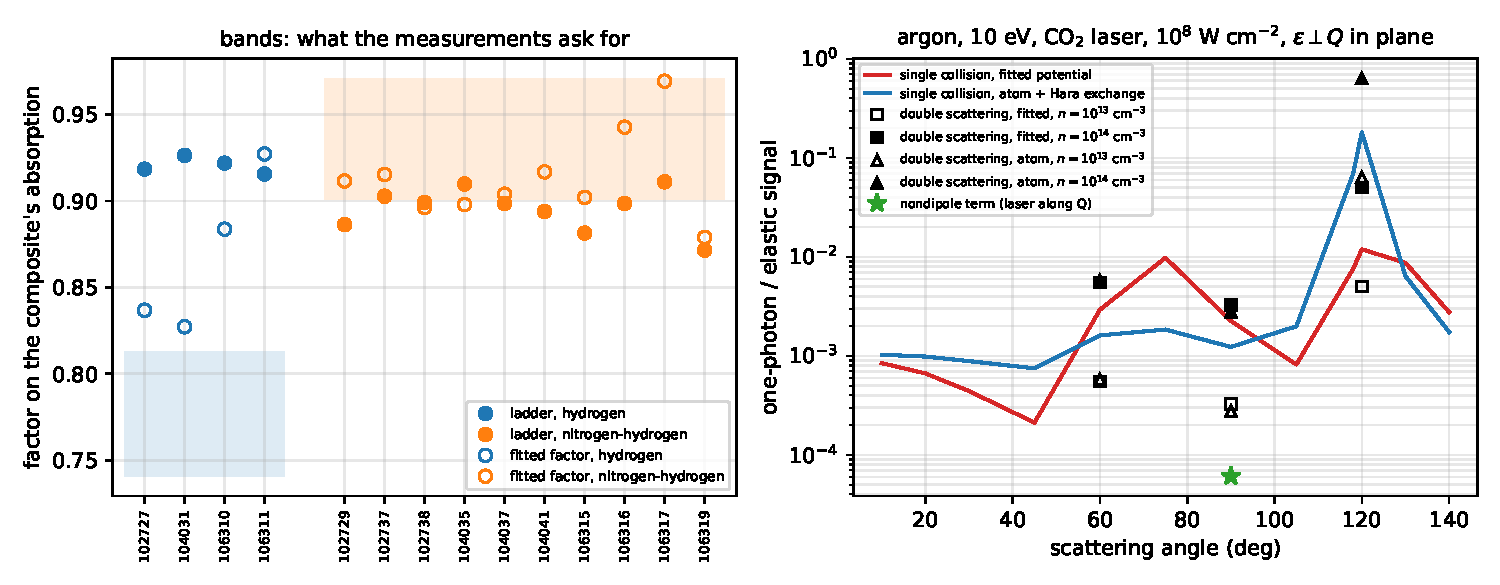
\includegraphics[width=\textwidth]{v3_fig.pdf}
\caption{Left: per shot, the factor $X$ of Eq.~(\ref*{eq:X}) that the ladder applies beyond the composite
of Turnbull et al.\ (filled) and their fitted screening factor $f_{sc}$ (open), against the factor the
measurements ask for, $1/(1.29\pm0.06)$ for hydrogen and $1/(1.07\pm0.04)$ for the mixtures (bands).
Right: argon at 10~eV in a CO$_2$ laser at $10^8$~W\,cm$^{-2}$, in the in-plane geometry with
$\boldsymbol\epsilon\perp\mathbf Q$: the exact single-collision one-photon signal relative to the elastic
one for the two potentials (lines), double scattering in the target at $10^{13}$ and $10^{14}$~cm$^{-3}$
(markers), and the nondipole term (star).}
\label{fig:v3}
\end{figure}

\subsection{Rules against counting an effect twice}
\label{sec:rules}
\begin{enumerate}
\item \emph{One upper cutoff.} The dynamic cutoff $v_t/\omega$ of Sec.~\ref{sec:quantum} and the Debye length of Sec.~\ref{sec:drude} are
two models of the same long-range cut. Electron screening enters through $\varepsilon$ in Sec.~\ref{sec:escreen}, never
as a second cutoff.
\item \emph{One account of the ions.} The rung of Sec.~\ref{sec:ions} and a fitted screening factor both describe how the ions
modify the long-range part of the logarithm. Applying $f_{sc}$ on top of that rung counts the ion
correlations twice.
\item \emph{Strong collisions once.} The exact Gaunt factor of Sec.~\ref{sec:strong} already contains the Born term;
it is added as $\Lambda_4-\Lambda_1$ to the medium logarithm, not multiplied by it, and the
cross term of Eq.~\eqref{eq:cross} is the only further piece.
\item \emph{One logarithm throughout.} The Langdon factor of Sec.~\ref{sec:langdon} must use the same velocity-dependent
logarithm as Sec.~\ref{sec:quantum} or \ref{sec:strong}; Langdon's fit alone assumes a fixed one.
\item \emph{The field once per beam.} $R_{\rm self}$ holds the probe's own quiver, $R_{pp}$ the
heaters'; the Langdon parameter $\alpha$ of Sec.~\ref{sec:langdon} takes the overlapped intensity because it describes
the time-averaged distribution, which every beam shapes. Neither replaces the other.
\item \emph{No separate term for collision sequences.} Double scattering is already in the
kinetic equation (Sec.~\ref{sec:multiple}).
\item \emph{Electron--electron collisions shape, they do not absorb.} They enter through $\alpha$ in
Sec.~\ref{sec:langdon} and through the relaxation of $f_2$ in Sec.~\ref{sec:aniso}, not as a third scatterer.
\item \emph{Two logarithms in the anisotropy.} The field drives $f_2$ with the inverse-bremsstrahlung
logarithm, and collisions relax it with the transport logarithm; using one for both overstates the
anisotropy by $\Lambda_{\rm tr}/\Lambda_1\approx1.5$.
\end{enumerate}

\section{Have the models improved?}
\label{sec:verdict}

{\noindent}\emph{Plasma.} Against the composite of Turnbull et al.\ without their screening factor,
which is $1.29\pm0.06$ times the measured absorption of the hydrogen shots and $1.07\pm0.04$ times
that of the mixture shots, the ladder is
\begin{equation}
\boxed{\;\frac{K_{\rm ladder}}{K_{\rm measured}}=
\begin{cases}
1.07\,\bar X_{\rm N_2/H_2}=1.07\times0.895=0.96\pm0.04 & \text{(ten nitrogen--hydrogen shots)},\\[2pt]
1.29\,\bar X_{\rm H_2}=1.29\times0.921=1.19\pm0.06 & \text{(four hydrogen shots)}.
\end{cases}\;}
\label{eq:verdict}
\end{equation}
For the mixtures the ladder, with no fitted parameter, agrees with the measurements as well as the
fitted composite of Turnbull et al., $1.00\pm0.04$ \cite{Turnbull2024}. In these plasmas the fitted
factor and the computed correlations of the ions do the same thing, 0.879 to 0.969 against a medium
factor of 0.930 to 0.982, because the heavy ions make the correlations strong. For hydrogen they part:
the fitted factor lowers the absorption by 7 to 17\,\%, the medium by 0.4 to 2.2\,\%, and the
hypernetted chain confirms Debye--H\"uckel to $2\times10^{-4}$ at $\Gamma_{ii}=0.02$. \emph{The ladder
explains the mixture shots and leaves the hydrogen shots 19\,\% too absorbing.} Every rung that
could act on hydrogen alone is now computed and small: the anisotropy, which scales as $1/Z$, 0.8 to
1.3\,\%; the strong fields 1 to 5\,\%; the speckles 2.3 to 4.5\,\%. The residual is the size of a 12\,\% error
in $T_e$ or a 9\,\% error in $n_e$ of the hydrogen shots, whose measured absorption, 0.15 to 1.48\,\%, is
the smallest of the data set (0.47 to 5.05\,\% for the mixtures).

{\noindent}\emph{The discriminating measurement.} Helium against hydrogen at the conditions of the
four hydrogen shots, each normalized by the unscreened model of its own charge: the ladder predicts
0.987, 0.985, 0.993 and 0.997, the fitted factor 1.042, 1.044, 1.034 and 1.024. The two differ by 2.7
to 5.8\,\% and move in opposite directions.

{\noindent}\emph{Gas.} Against a Drude model with a mean collision frequency,
\begin{equation}
\boxed{\;\frac{K_{\rm ladder}}{K_{\rm Drude}}=\frac{\langle\nu_m\,2\varepsilon/3\kB T_e\rangle}{\langle\nu_m\rangle}\,R
=0.836\ \text{(300 K)}\ \text{to}\ 2.02\ \text{(1.08 eV)}\ \text{at 1 to 4 THz},\;}
\label{eq:verdictgas}
\end{equation}
where $R$ of Secs.~\ref{sec:phases} and \ref{sec:polbrems} is 0.97 to 1.00 at 1 to 4~THz, and at 28.3~THz $R$ lowers it further, to 0.514
of the classical kernel for 300~K electrons with the fitted potential and 0.491 with the potential
from the atom (Table~\ref{tab:gas}). The single collisions beyond Kroll and Watson are computed
(Table~\ref{tab:onetwo}); they equal double scattering at the densities of the targets used.

\section{What remains open}
\label{sec:open}

\begin{enumerate}
\item \emph{The hydrogen residual.} The ladder accounts for the mixture shots and leaves 19\,\% for
hydrogen, with every hydrogen-specific rung computed. The theory therefore places the residual in
the hydrogen measurements or their plasma conditions, not in the absorption physics; the helium
measurement of Sec.~\ref{sec:verdict} decides between this and a fitted screening length.
\item \emph{The anisotropy beyond its direct part.} The feedback of $f_2$ on the isotropic
distribution and the field-particle part of the electron--electron operator are not computed. They
change the 0.8 to 1.3\,\% of Sec.~\ref{sec:aniso} by a factor of order one, not the residual.
\item \emph{Argon at the elastic minima.} The single-collision and double-scattering signals are
computed; near the minima of the elastic cross section, where the measured photon exchange is
largest, both depend on the depth and the position of the minimum, which the two potentials do not
agree on. A density scan in the in-plane and normal geometries measures both.
\end{enumerate}
Closed here: the ion correlations beyond Debye--H\"uckel (Sec.~\ref{sec:ions}), the strong-collision cross
term at the mixtures' conditions (Sec.~\ref{sec:strong}), the heaters' own strong-field factor and the exact factor at
$\beta\ge1$ (Sec.~\ref{sec:fields}), the anisotropy with two logarithms and electron--electron collisions (Sec.~\ref{sec:aniso}), and the
single-collision photon exchange beyond Kroll and Watson in argon (Sec.~\ref{sec:onetwo}).

\begin{thebibliography}{99}
\raggedright
\bibitem{Atzeni2004} S.~Atzeni and J.~Meyer-ter-Vehn, \emph{The Physics of Inertial Fusion}
(Oxford University Press, Oxford, 2004), doi:\href{https://doi.org/10.1093/acprof:oso/9780198562641.001.0001}{10.1093/acprof:oso/9780198562641.001.0001}.
\bibitem{Turnbull2023} D.~Turnbull \emph{et al.}, Phys. Rev. Lett. \textbf{130}, 145103 (2023),
doi:\href{https://doi.org/10.1103/PhysRevLett.130.145103}{10.1103/PhysRevLett.130.145103}.
\bibitem{Turnbull2024} D.~Turnbull \emph{et al.}, Phys. Plasmas \textbf{31}, 063304 (2024),
doi:\href{https://doi.org/10.1063/5.0203446}{10.1063/5.0203446}.
\bibitem{Kramers1923} H.~A.~Kramers, Phil. Mag. \textbf{46}, 836 (1923),
doi:\href{https://doi.org/10.1080/14786442308565244}{10.1080/14786442308565244}.
\bibitem{KarzasLatter1961} W.~J.~Karzas and R.~Latter, Astrophys. J. Suppl. \textbf{6}, 167 (1961),
doi:\href{https://doi.org/10.1086/190063}{10.1086/190063}.
\bibitem{DawsonOberman1962} J.~Dawson and C.~Oberman, Phys. Fluids \textbf{5}, 517 (1962),
doi:\href{https://doi.org/10.1063/1.1706652}{10.1063/1.1706652}.
\bibitem{Sommerfeld1931} A.~Sommerfeld, Ann. Phys. \textbf{403}, 257 (1931),
doi:\href{https://doi.org/10.1002/andp.19314030302}{10.1002/andp.19314030302}.
\bibitem{vanHoof2014} P.~A.~M.~van~Hoof, R.~J.~R.~Williams, K.~Volk, M.~Chatzikos, G.~J.~Ferland,
M.~Lykins, R.~L.~Porter and Y.~Wang, Mon. Not. R. Astron. Soc. \textbf{444}, 420 (2014),
doi:\href{https://doi.org/10.1093/mnras/stu1438}{10.1093/mnras/stu1438}.
\bibitem{Bloch1933} F.~Bloch, Ann. Phys. (Leipzig) \textbf{408}, 285 (1933),
doi:\href{https://doi.org/10.1002/andp.19334080303}{10.1002/andp.19334080303}.
\bibitem{Langdon1980} A.~B.~Langdon, Phys. Rev. Lett. \textbf{44}, 575 (1980),
doi:\href{https://doi.org/10.1103/PhysRevLett.44.575}{10.1103/PhysRevLett.44.575}.
\bibitem{Matte1988} J.~P.~Matte, M.~Lamoureux, C.~M\"oller, R.~Y.~Yin, J.~Delettrez, J.~Virmont
and T.~W.~Johnston, Plasma Phys. Control. Fusion \textbf{30}, 1665 (1988),
doi:\href{https://doi.org/10.1088/0741-3335/30/12/004}{10.1088/0741-3335/30/12/004}.
\bibitem{KullPlagne2001} H.-J.~Kull and L.~Plagne, Phys. Plasmas \textbf{8}, 5244 (2001),
doi:\href{https://doi.org/10.1063/1.1416182}{10.1063/1.1416182}.
\bibitem{Bornath2001} Th.~Bornath, M.~Schlanges, P.~Hilse and D.~Kremp, Phys. Rev. E \textbf{64},
026414 (2001), doi:\href{https://doi.org/10.1103/PhysRevE.64.026414}{10.1103/PhysRevE.64.026414}.
\bibitem{Decker1994} C.~D.~Decker, W.~B.~Mori, J.~M.~Dawson and T.~Katsouleas, Phys. Plasmas
\textbf{1}, 4043 (1994), doi:\href{https://doi.org/10.1063/1.870874}{10.1063/1.870874}.
\bibitem{Alves2014} L.~L.~Alves, J. Phys.: Conf. Ser. \textbf{565}, 012007 (2014),
doi:\href{https://doi.org/10.1088/1742-6596/565/1/012007}{10.1088/1742-6596/565/1/012007};
IST-Lisbon database, \url{https://www.lxcat.net}.
\bibitem{Yamabe1983} C.~Yamabe, S.~J.~Buckman and A.~V.~Phelps, Phys. Rev. A \textbf{27}, 1345 (1983),
doi:\href{https://doi.org/10.1103/PhysRevA.27.1345}{10.1103/PhysRevA.27.1345}.
\bibitem{Pitchford2016} L.~C.~Pitchford \emph{et al.}, Plasma Process. Polym. \textbf{14}, 1600098
(2016), doi:\href{https://doi.org/10.1002/ppap.201600098}{10.1002/ppap.201600098}.
\bibitem{Low1958} F.~E.~Low, Phys. Rev. \textbf{110}, 974 (1958),
doi:\href{https://doi.org/10.1103/PhysRev.110.974}{10.1103/PhysRev.110.974}.
\bibitem{KrollWatson1973} N.~M.~Kroll and K.~M.~Watson, Phys. Rev. A \textbf{8}, 804 (1973),
doi:\href{https://doi.org/10.1103/PhysRevA.8.804}{10.1103/PhysRevA.8.804}.
\bibitem{GSZ1969} A.~E.~S.~Green, D.~L.~Sellin and A.~S.~Zachor, Phys. Rev. \textbf{184}, 1 (1969),
doi:\href{https://doi.org/10.1103/PhysRev.184.1}{10.1103/PhysRev.184.1}.
\bibitem{Schwerdtfeger2019} P.~Schwerdtfeger and J.~K.~Nagle, Mol. Phys. \textbf{117}, 1200 (2019),
doi:\href{https://doi.org/10.1080/00268976.2018.1535143}{10.1080/00268976.2018.1535143}.
\bibitem{FurnessMcCarthy1973} J.~B.~Furness and I.~E.~McCarthy, J. Phys. B: At. Mol. Phys. \textbf{6},
2280 (1973), doi:\href{https://doi.org/10.1088/0022-3700/6/11/021}{10.1088/0022-3700/6/11/021}.
\bibitem{Hara1967} S.~Hara, J. Phys. Soc. Jpn. \textbf{22}, 710 (1967),
doi:\href{https://doi.org/10.1143/JPSJ.22.710}{10.1143/JPSJ.22.710}.
\bibitem{WallbankHolmes1994} B.~Wallbank and J.~K.~Holmes, J. Phys. B: At. Mol. Opt. Phys.
\textbf{27}, 5405 (1994),
doi:\href{https://doi.org/10.1088/0953-4075/27/21/027}{10.1088/0953-4075/27/21/027}.
\bibitem{Rabadan1996} I.~Rabad\'an, L.~M\'endez and A.~S.~Dickinson, J. Phys. B: At. Mol. Opt. Phys.
\textbf{29}, L801 (1996),
doi:\href{https://doi.org/10.1088/0953-4075/29/22/004}{10.1088/0953-4075/29/22/004}.
\bibitem{Morita1958} T.~Morita, Prog. Theor. Phys. \textbf{20}, 920 (1958),
doi:\href{https://doi.org/10.1143/PTP.20.920}{10.1143/PTP.20.920}.
\bibitem{Slattery1982} W.~L.~Slattery, G.~D.~Doolen and H.~E.~DeWitt, Phys. Rev. A \textbf{26}, 2255 (1982),
doi:\href{https://doi.org/10.1103/PhysRevA.26.2255}{10.1103/PhysRevA.26.2255}.
\bibitem{Abe1959} R.~Abe, Prog. Theor. Phys. \textbf{22}, 213 (1959),
doi:\href{https://doi.org/10.1143/PTP.22.213}{10.1143/PTP.22.213}.
\bibitem{Rosenbluth1957} M.~N.~Rosenbluth, W.~M.~MacDonald and D.~L.~Judd, Phys. Rev. \textbf{107}, 1 (1957),
doi:\href{https://doi.org/10.1103/PhysRev.107.1}{10.1103/PhysRev.107.1}.
\bibitem{Spitzer1953} L.~Spitzer and R.~H\"arm, Phys. Rev. \textbf{89}, 977 (1953),
doi:\href{https://doi.org/10.1103/PhysRev.89.977}{10.1103/PhysRev.89.977}.
\bibitem{OMalley1961} T.~F.~O'Malley, L.~Spruch and L.~Rosenberg, J. Math. Phys. \textbf{2}, 491 (1961),
doi:\href{https://doi.org/10.1063/1.1703735}{10.1063/1.1703735}.
\end{thebibliography}

\end{document}
